\documentclass[prX,nofootinbib,notitlepage]{revtex4-1}

% For two-column format (which usually looks more professional):
%\documentclass[twocolumn,prX,nofootinbib,notitlepage]{revtex4-1}

% Note: The revtex4-1 document class includes a variety of Physics Journal
% styles. The option prX is specifies the Physical Review X journal style.


%*************************** Load Packages *******************************
% Note: Package descriptions and usage documentation can be found online
% at https://ctan.org/. Just use the site's search bar to search for the
% package

%------------------ Extending default LaTeX Structures -------------------
\usepackage{enumerate}
\usepackage{float}
\usepackage{caption}
\usepackage{hyperref}
\usepackage{subfiles}

%------------------------ Symbology \& Math ------------------------------
\usepackage{amsmath, amsthm, amssymb, amsfonts}
\usepackage{mathrsfs}
\usepackage{array}

%--------------------------- Graphics ------------------------------------
\usepackage[dvips]{graphics}
\usepackage{graphicx}
\usepackage{color}

\usepackage{enumitem}


\begin{document}
\bibliographystyle{plain}

\title{PHYS 506 - Experiment 3}

%----------------------- Author Information ------------------------------
\author{Luke Abanilla}%
\author{Eben Quenneville}
\author{Augustus Vigorito}
\affiliation{Department of Physics, University of New Hampshire,
Durham, NH 03824, USA}
\date{December 2024}

\maketitle
\vspace{-8cm}

\section{Experimental Methods}

\textbf{Write about the experimental procedure and methods of this lab experiment, as if you were writing the Experimental Methods section of a formal lab report. (The mock-up experimental methods section should probably be two or more paragraphs).}

\textbf{Recall that the role of an Experimental Methods section is to give a description of the experiment you carried out. Write in your own words, but also try to maintain an air of formality in your writing. The experimental setup should not be a step-by-step recipe, but, rather, a set of text that describes all the various pieces of equipment used (ideally with diagrams, technical drawings, and/or circuit schematics), their arrangements, any calibrations, any settings, how the data was collected, and other information deemed necessary for the reader to understand what you did in this experiment.}

In this experiment, we used two instruments to gather data about photocurrent as a function of stopping voltage: the Model P67401, hereafter referred to interchangeably as the analog instrument, and the Model PLCN01, or digital instrument. In general terms, these apparatus work by having a light source set up opposite a collimating tube with a filter at the entrance. The light source is turned on and photons of a certain wavelength pass through the filter, where they encounter an accelerating voltage. Photons with enough energy reach the cathode of the phototube, where they eject electrons and create a current through a picoamplifier. Our experiment was to measure the current induced by these ejected electrons for various wavelength filters and accelerating voltages, using both analog and digital instruments.

The first step with either instrument is to gather data about the dark characteristic current - that is, the current measured by the instrument when the collimating light tube is blocked off and therefore no photons should be reaching the cathode of the phototube. We found for the digital instrument that blocking off the light stopped the current completely, making the dark characteristic curve 0. For the analog instrument, we had to first calibrate the instrument. This is done by adjusting the range to make the ammeter read 0 on both its short and full range scale settings. Then, we placed the cover over the phototube and measured the dark current for various accelerating voltages. We found that it wasn't quite all 0, as we had seen with the digital apparatus. The dark current was on the order of $10^{-14}~\text{A}$. With this calibration step out of the way, we were ready to gather data.

The digital instrument measured currents up to a maximum magnitude of 2 nanoamps. For each wavelength filter, we began taking our measurements at an accelerating voltage that induced a current close to -2 nanoamps, and then used the potentiometer to step up the voltage in small increments of $0.05~\text{V}$. We continued increasing the voltage until reaching what appeared to be the saturation current value (that is, when increasing the accelerating voltage no longer increased the current). For the analog apparatus, we always began at an accelerating voltage of $-2~\text{V}$ and then increased in slightly more coarse voltage steps of $0.2~\text{V}$ until we saw significant changes in the current, at which point we began changing the voltage by steps of $0.025~\text{V}$. We repeated this until reaching the minimum accelerating voltage for this apparatus of $0~\text{V}$. We analyze the results of this experiment in the following section. 

\pagebreak

\section{Data Visualization}

% \underline{add the plots as numbered figures with brief descriptive captions}

\begin{figure}[ht!]
    \centering
    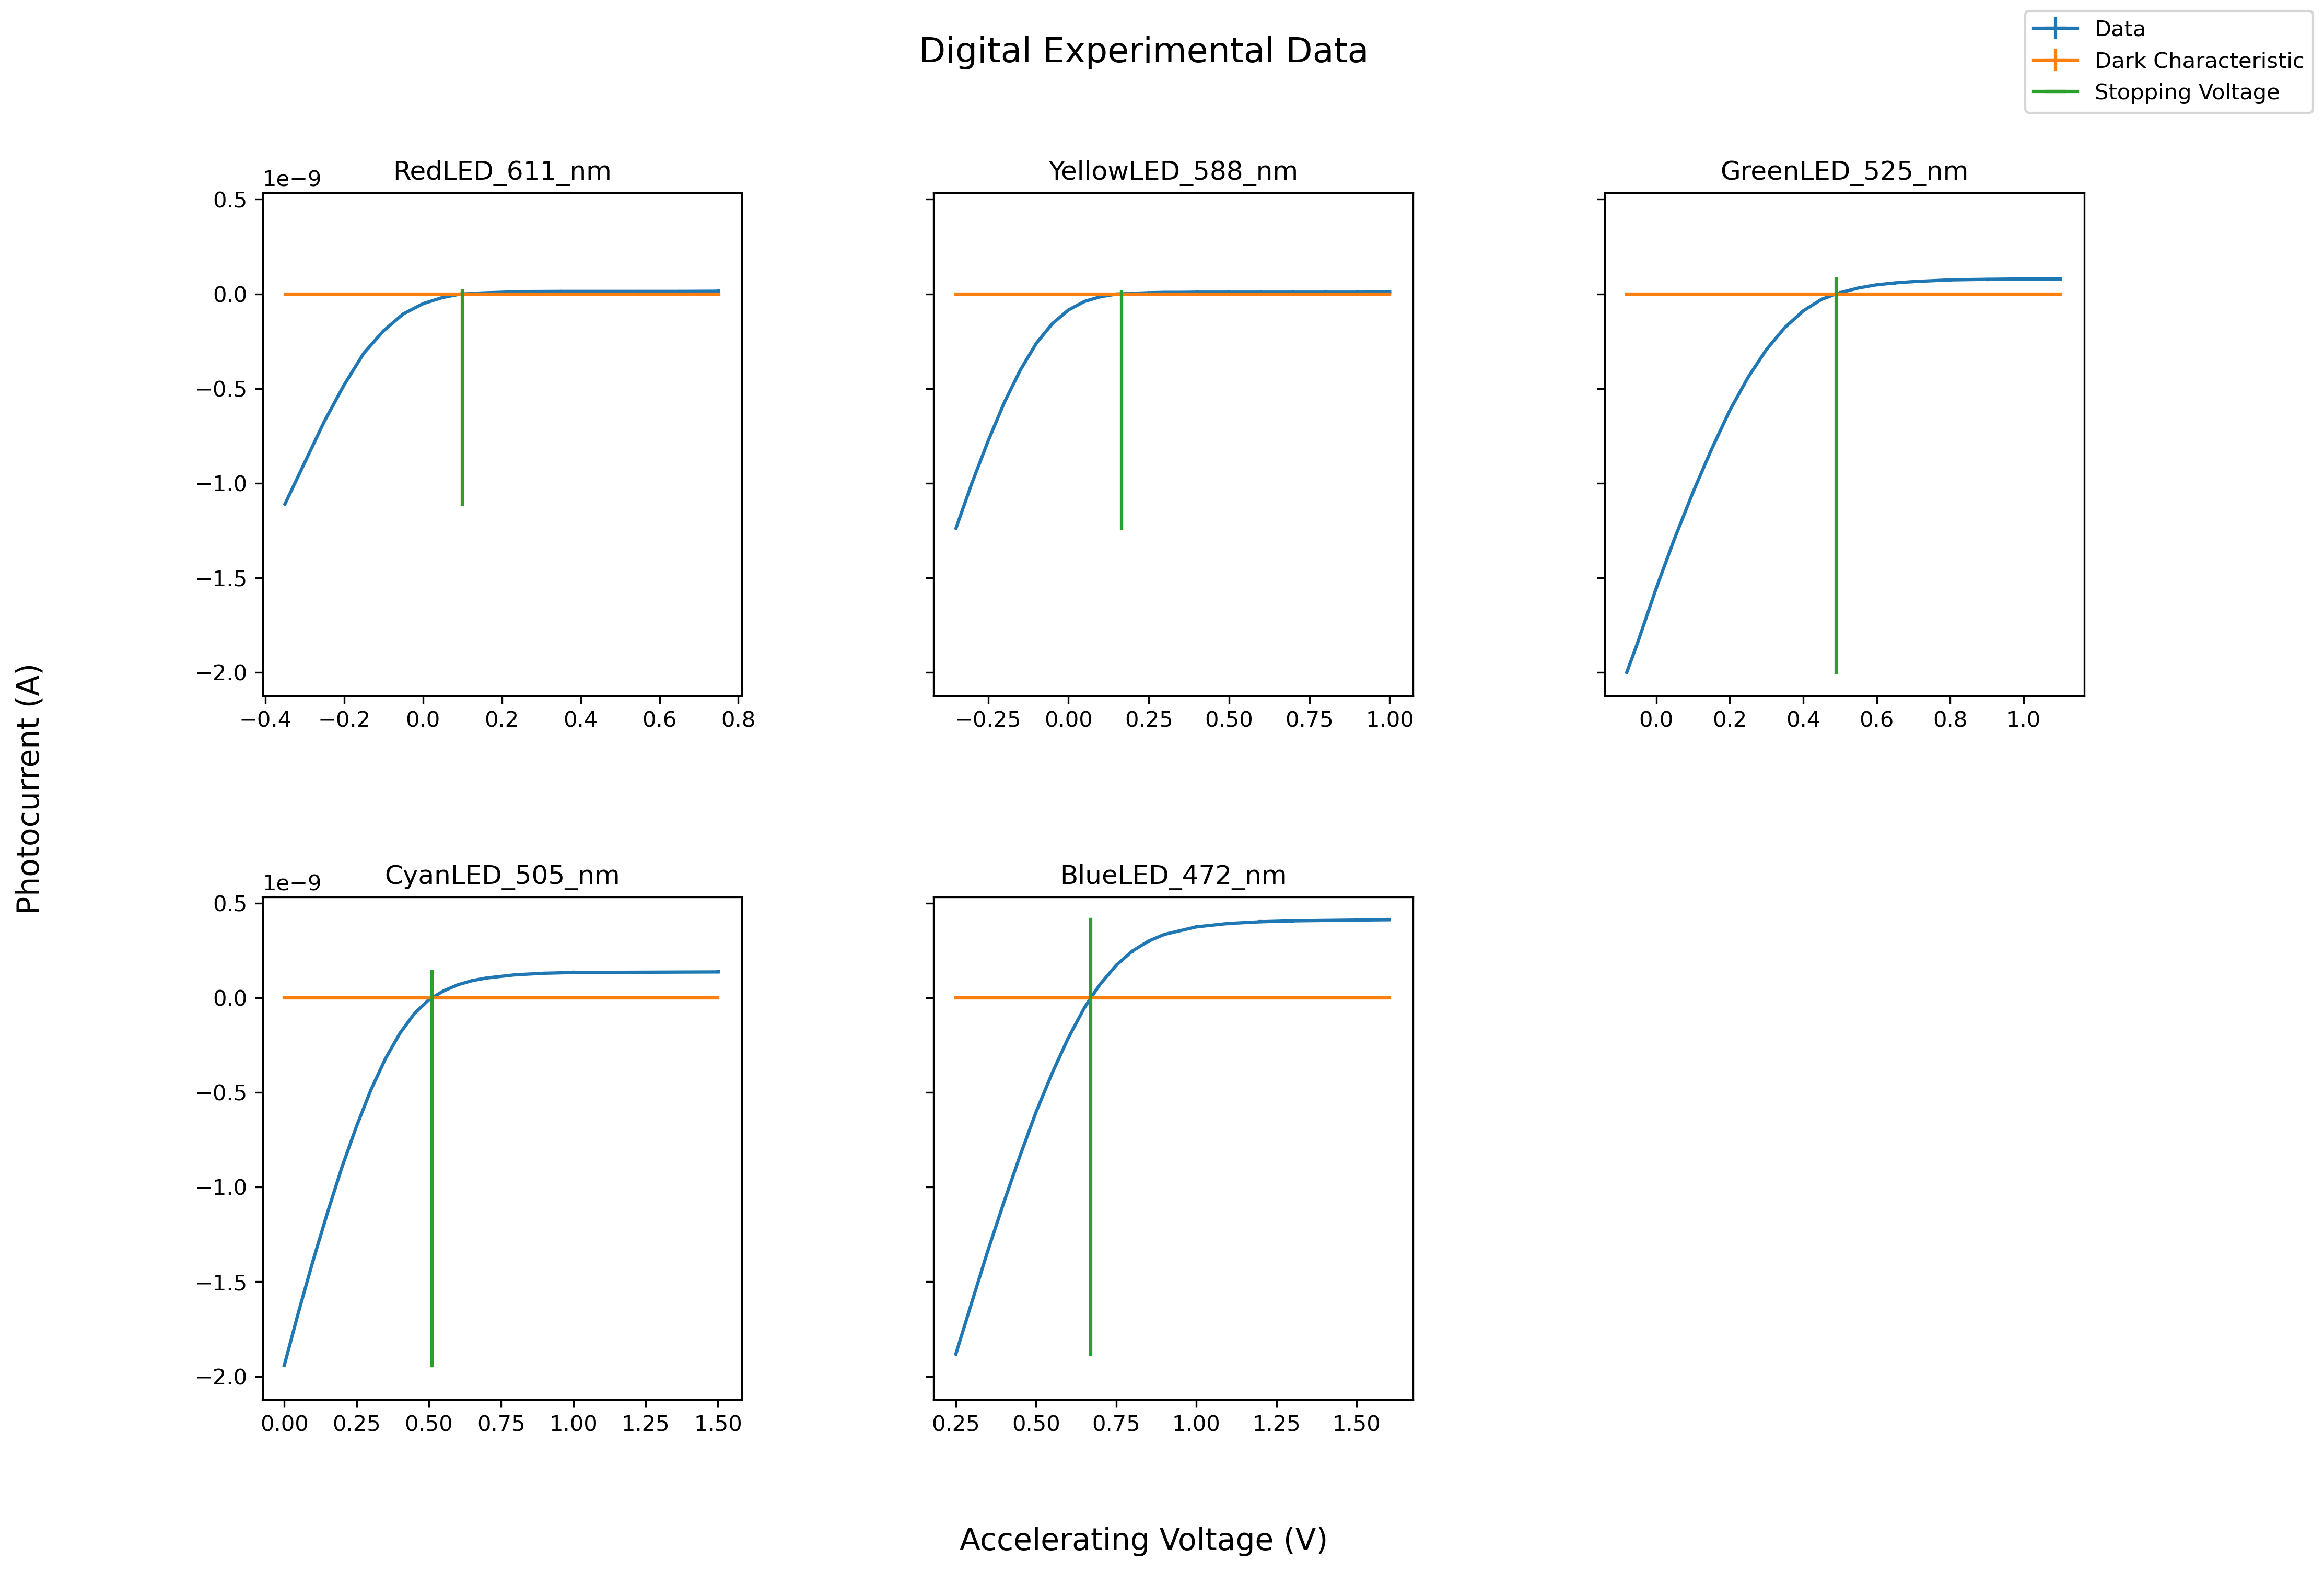
\includegraphics[width=0.75\linewidth]{Digital_Data_2x3.png}
    \caption{Graph of Model PLCN01 Voltage vs. Photocurrent Data for Five Different Wavelength Filters}
    \label{fig:digital_data}
    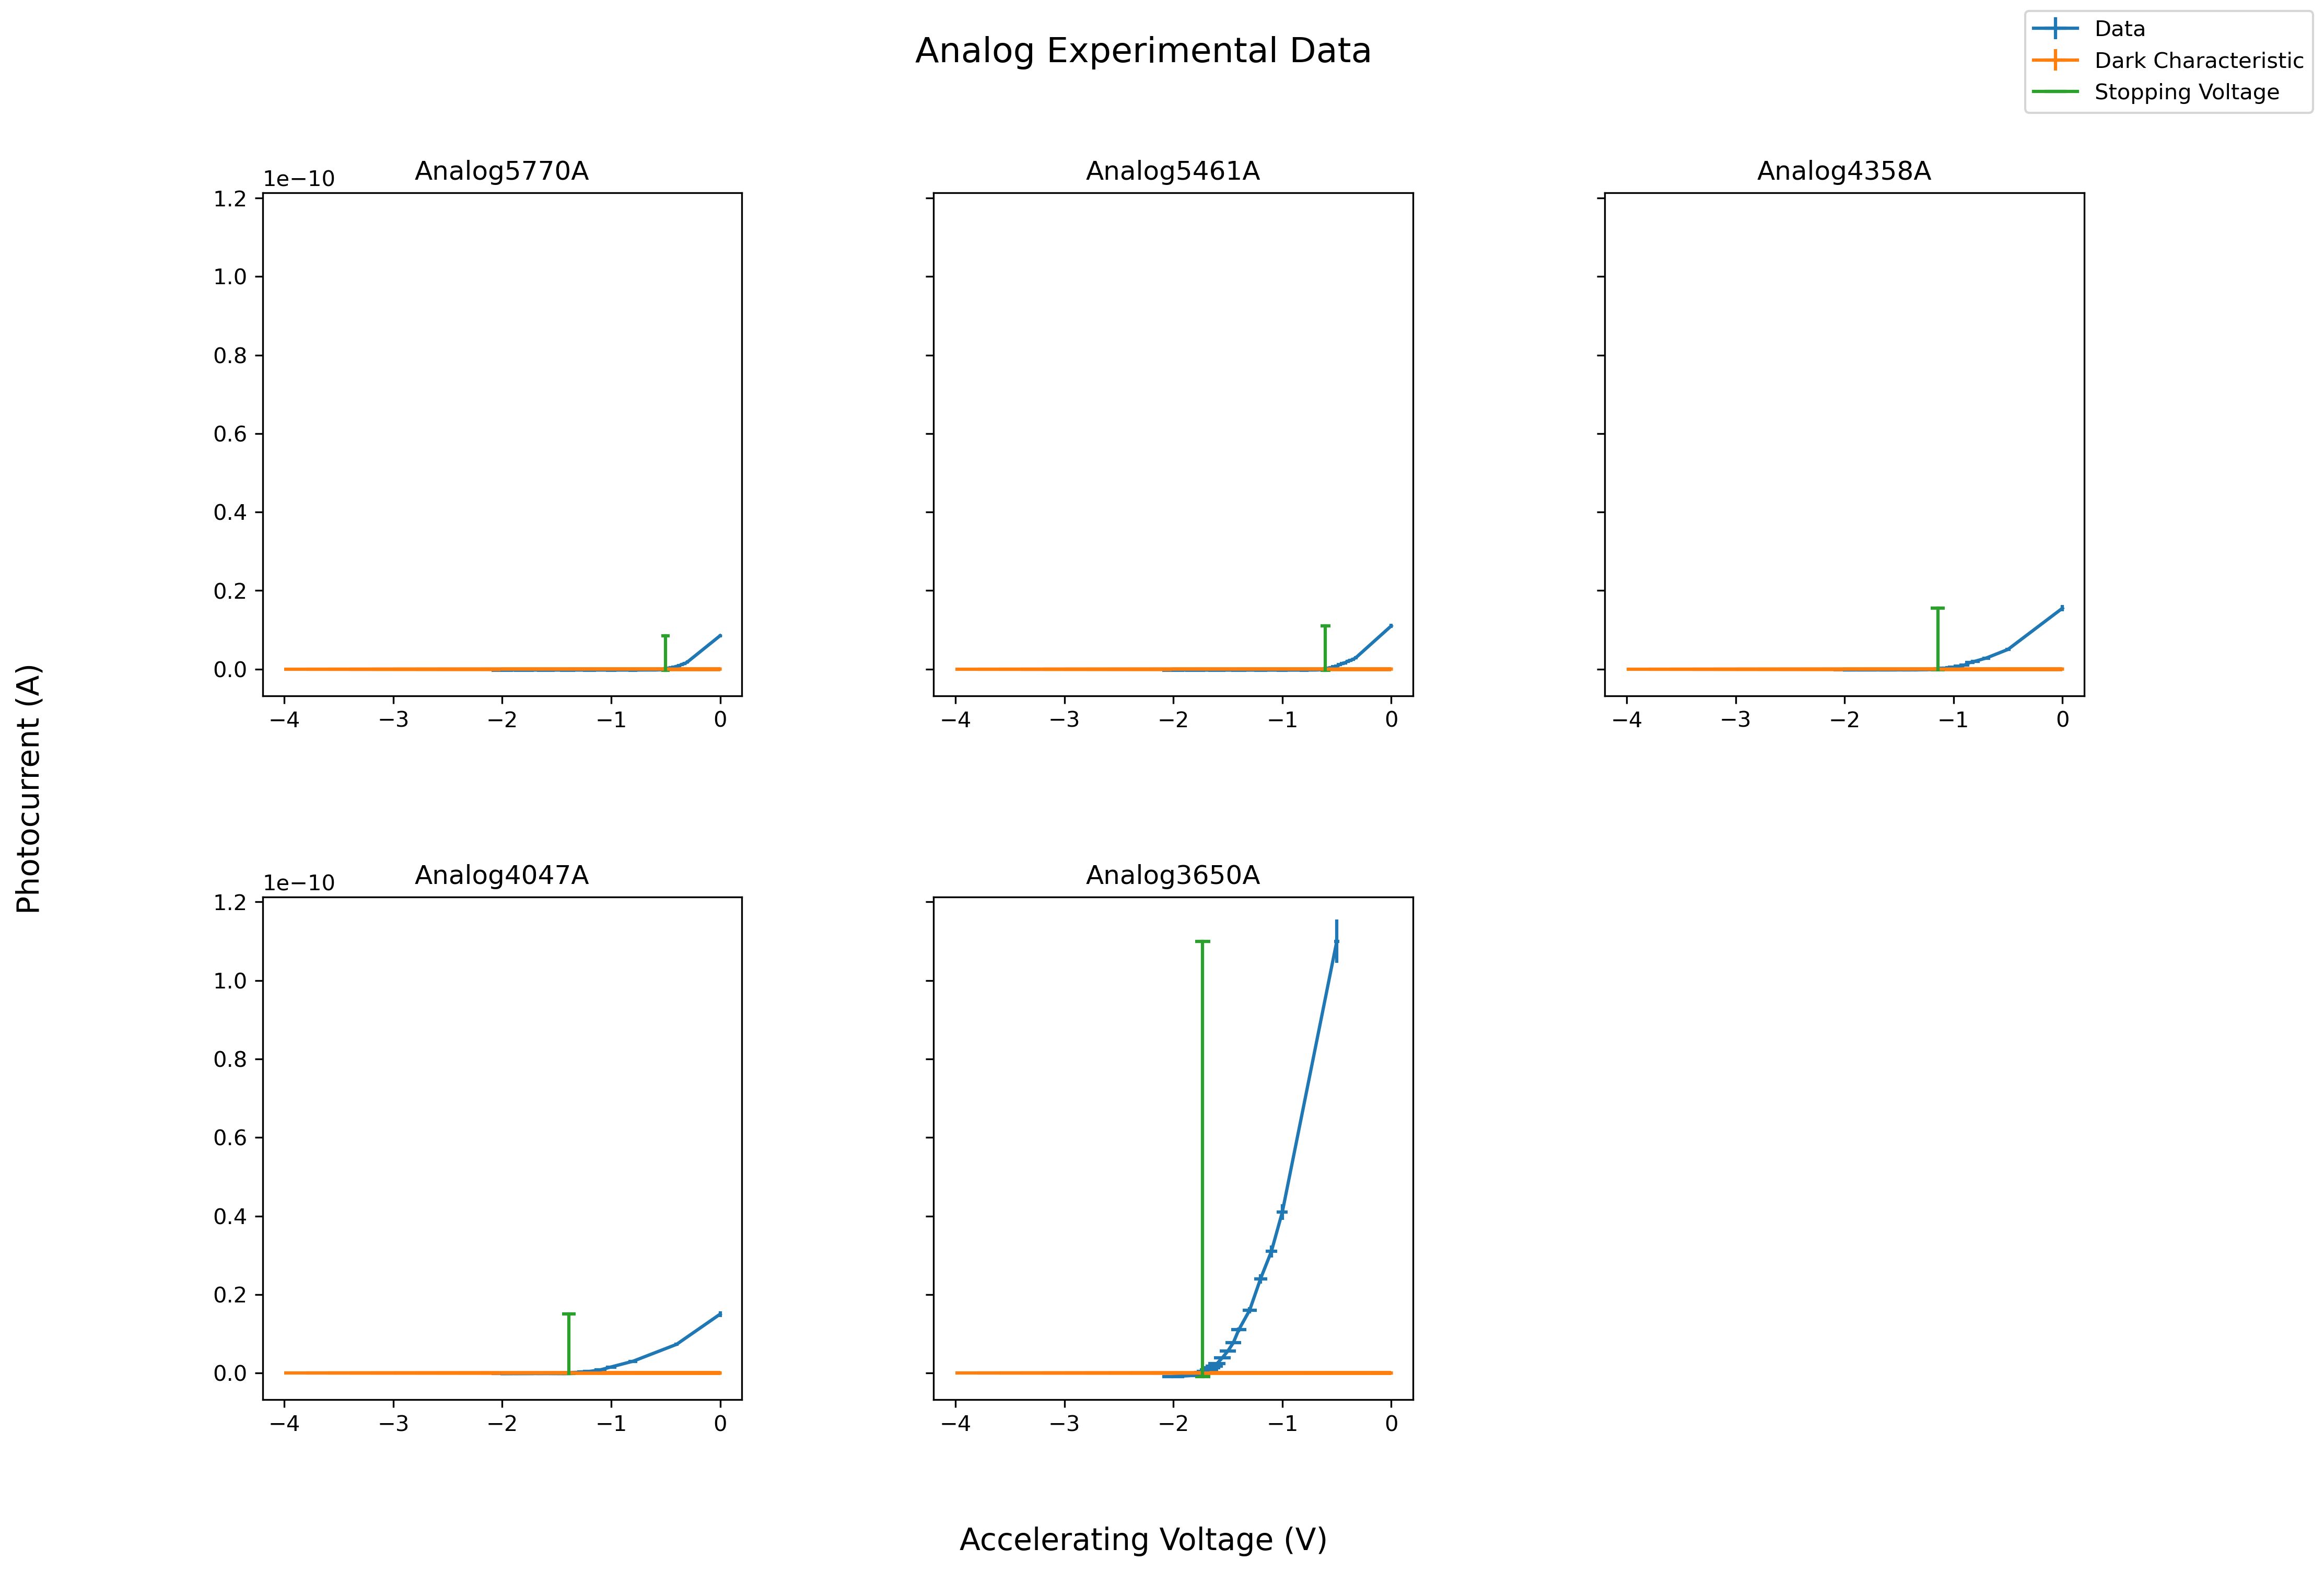
\includegraphics[width=0.75\linewidth]{Analog_Data_2x3.png}
    \caption{Graph of Model 67401 Voltage vs. Photocurrent Data for Five Different Wavelength Filters}
    \label{fig:analog_data}
\end{figure}

\pagebreak
\section{Results and Analysis}

\textbf{Display your plot of stopping potential versus frequency of incident light as a numbered figure with a descriptive caption. Make sure your plot has labeled axes, error bars, and a fit line. Below your figure, wirte a paragraph which refers to, discusses, and explains the figure. This discussion should include:}
\begin{itemize}
    \item An explanation of how you obtained the stopping potentials 
    \item An explanation of how uncertainties were determined
    \item An explanation of the role of the fit line, and how the fit line was determined
    \item Anything else that you deem relevant in describing how the data you took in Problem 1 became the stopping potential vs. frequency plot you are presenting here, and how you used this plot to find a value for Planck's constant h. 
\end{itemize}

\begin{figure}[ht]
    \centering
    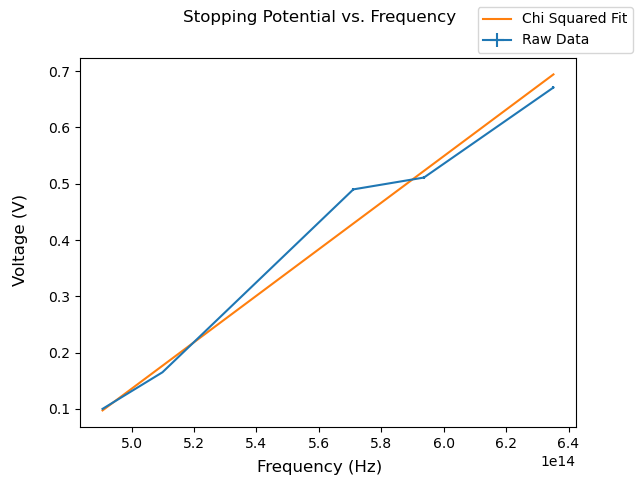
\includegraphics[width=0.75\linewidth]{Stopping_Potential.png}
    \caption{Graph of Stopping Potential vs. Frequency using the P67401 apparatus data}
    \label{fig:stopping_potential}
\end{figure}

In this figure, we see a representation of the stopping voltage in Volts versus the frequency of incident light in Hz. Many steps went into generating this plot.
Using the PLCN01 apparatus, we collected a series of current and voltage data points based on the photoelectric effect. Each data point gave the number of electrons with sufficient kinetic energy to overcome a given voltage, as measured by the induced current, for a given light source and filter. We collected five series of data: one for each of five different wavelength filters, as seen in \ref{fig:digital_data}. We additionally collected a dark characteristic current (the measurement of the apparatus with no incident light). This was 0, represented by the orange line in \ref{fig:digital_data}. The stopping voltage, $V_S$, is the voltage at which the current is equal to the dark characteristic current (and therefore no electrons have sufficient kinetic energy to overcome the potential barrier). To find $V_S$ from our data using a generically applicable method, we took the current measurement at each voltage and shifted it by the average of the two nearest data points in the dark characteristic curve. Then, we found the point at which this shifted current curve passed the $I=0$ line (the horizontal axis in \ref{fig:digital_data}) by averaging the two shifted data points closest to the line. To find the uncertainty of this calculated value, we carefully stepped through the algorithm to come up with a mathematical formula representing the stopping voltage, given as
$$V_{S} = \frac{m_{D} V_{D1} - m_{L} V_{L1} + C_{L1} - C_{D1}}{m_{D} - m_{L}}$$

where $V_S$ is the stopping voltage, $m_D = \frac{C_{D1} - C_{D2}}{V_{D1} - V_{D2}}$ is the slope of the dark characteristic curve in the region of interest, $m_L = \frac{C_{L1} - C_{L2}}{V_{L1} - V_{L2}}$ is the slope of the light curve, and the points $V_{D1}, ~ V_{D2}, \dots$ are the voltage and current data points of the dark and light curves near the root. The uncertainty is then found using multivariable uncertainty propagation, as is typical. The full details can be seen in the Python code. 

With the stopping voltages found for each characteristic wavelength, we can then produce \ref{fig:stopping_potential} by using the relationship that $c = \lambda f$ for light. For each wavelength, we can calculate the corresponding frequency as
$$
f = \frac{c}{\lambda}; \quad \delta f = \sqrt{(- \frac{c}{\lambda^{2}} \delta \lambda)^{2}}
$$
when we assume that the uncertainty in the speed of light is 0. We further assumed that the uncertainty in the wavelength of the filters was $5\%$. Applying this mathematical analysis to our five different wavelength filters gives us five data points of wavelength versus stopping voltage. Then, to find the slope between them, we applied a chi-squared fit without dependence on $x$-uncertainty. This linear regression algorithm aims to minimize the difference of the squares between each data point and the line of best fit but also weighs each data point according to the uncertainty associated with that measurement. The resulting line of best fit, $V_{S} = mf + b$, is displayed in \ref{fig:stopping_potential} in orange. It can be shown through physics first principles that the line shown in that figure is representative of the equation. 
$$
V_{S} = \frac{h}{e} f - \frac{\phi}{e}
$$
where $h$ is Planck's constant, $e$ is the elementary charge of an electron, and $\phi$ is the work function of the material. Our experimental value of $h$ is therefore given as 
$$
\boxed{h = \frac{b}{e} = 6.62 \times 10^{-34} ~ \text{J*s}; \quad \delta h = \sqrt{e^{2} \delta m^2  + m^2 \delta e^2} = 0.02 \times 10^{-34} ~ \text{J*s}}
$$





\section{General Data Presentation Considerations}

\textbf{What do you think is the best way to represent data in a formal lab report? (e.g. tables, plots, some combination) Explain and defend your reasoning in a few sentences.}

Data comes in many forms and can be presented in many more. The most appropriate way to represent data depends on your goals and audience. In general terms, graphical plots are the most effective way to concisely convey information. They are inherently visual, which engages the audience in a way that a table of data cannot. When you are reading an article, a striking figure or an informative plot is what you will remember more than any text. Tables, on the other hand, are ideal for presenting precise numerical values, uncertainties, or comparisons that may not be immediately clear from a plot. Both have their purposes in a formal lab report.

\end{document}